From our initial computational model, we would like for there to be a variety of uses for the Turing Machine. While implementing this, we run into a rather striking problem; the time taken for computations for larger languages grows considerably.

Increasing the size of the alphabet is not feasible, so we instead introduce a DTM on multiple tapes. These have separate read and write heads, though there is still only one finite state control.

\begin{figure}[h]
\centering
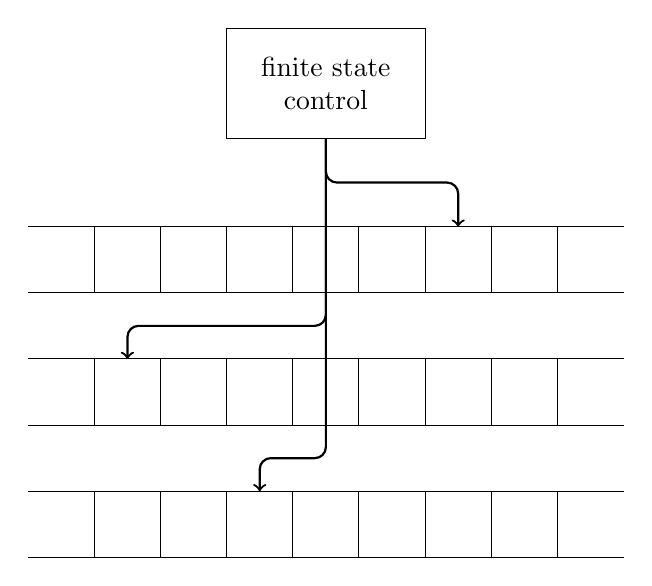
\begin{tikzpicture}[scale=1.4]
    \draw (5.5,1) rectangle (7.3,2);
    
    \node[text width = 2cm, align = center] at (6.4,1.5) {finite state control};

%Tape heads

    \draw[thick] [->] {[rounded corners] (6.4,1) -- (6.4,0.6) -- (7.6,0.6) -- (7.6,0.2)};

    \draw[thick] [->] {[rounded corners] (6.4,1) -- (6.4,-0.7) -- (4.6,-0.7) -- (4.6,-1)};

    \draw[thick] [->] {[rounded corners] (6.4,1) -- (6.4,-1.9) -- (5.8,-1.9) -- (5.8,-2.2)};

% First row of TM squares

	\draw (3.7,0.2) -- (4.3,0.2) -- (4.3,-0.4) -- (3.7,-0.4);
	\draw (4.3,0.2) rectangle (4.9,-0.4);
	\draw (4.9,0.2) rectangle (5.5,-0.4);
	\draw (5.5,0.2) rectangle (6.1,-0.4);
	\draw (6.1,0.2) rectangle (6.7,-0.4);
	\draw (6.7,0.2) rectangle (7.3,-0.4);
	\draw (7.3,0.2) rectangle (7.9,-0.4);
	\draw (7.9,0.2) rectangle (8.5,-0.4);
	\draw (9.1,-0.4) -- (8.5,-0.4) -- (8.5,0.2) -- (9.1,0.2);

%%Second row of TM squares
    \draw (3.7,-1) -- (4.3,-1) -- (4.3,-1.6) -- (3.7,-1.6);
	\draw (4.3,-1) rectangle (4.9,-1.6);
	\draw (4.9,-1) rectangle (5.5,-1.6);
	\draw (5.5,-1) rectangle (6.1,-1.6);
	\draw (6.1,-1) rectangle (6.7,-1.6);
	\draw (6.7,-1) rectangle (7.3,-1.6);
	\draw (7.3,-1) rectangle (7.9,-1.6);
	\draw (7.9,-1) rectangle (8.5,-1.6);
	\draw (9.1,-1.6) -- (8.5,-1.6) -- (8.5,-1) -- (9.1,-1);

%Third row of TM squares
    \draw (3.7,-2.2) -- (4.3,-2.2) -- (4.3,-2.8) -- (3.7,-2.8);
	\draw (4.3,-2.2) rectangle (4.9,-2.8);
	\draw (4.9,-2.2) rectangle (5.5,-2.8);
	\draw (5.5,-2.2) rectangle (6.1,-2.8);
	\draw (6.1,-2.2) rectangle (6.7,-2.8);
	\draw (6.7,-2.2) rectangle (7.3,-2.8);
	\draw (7.3,-2.2) rectangle (7.9,-2.8);
	\draw (7.9,-2.2) rectangle (8.5,-2.8);
	\draw (9.1,-2.8) -- (8.5,-2.8) -- (8.5,-2.2) -- (9.1,-2.2);    


\end{tikzpicture}


\caption{A $3$-tape DTM. The tape heads all move independently, but the DTM only works in one state at any time.}
\end{figure}

\newpage
\begin{definition}
    A program in a $k$-tape DTM is a tuple $(\Gamma,Q,\delta)$ such that:
    \begin{itemize}
        \item $\Gamma$ is a finite set of tape symbols, including a subset $\Sigma \subset \Gamma$ of input symbols and a unique blank symbol $b \in \Gamma \setminus \Sigma$;
        \item $Q$ is a finite set of states, including a unique start-state $q_0$ and two unique halt-states $q_Y$ and $q_N$;
        \item $\delta$ represents a transition function $\delta: Q \setminus \{q_Y,q_N\} \times \Gamma^k \to Q \times \Gamma^k \times \{-1,0,1\}^k$.
    \end{itemize}
\end{definition}

We note that Definition \ref{def:Computation} also holds for a $k$-tape DTM, and therefore we do not need to redefine computation on such machines. We motivate the importance of existence of $k$-tape DTMs with the following example, which computes on 2 tapes.

\begin{example}
    (Palindrome checker) Consider the following decision problem:
    
    \decisionproblem{Palindrome}{A string $x \in \{0,1\}^*$.}{Is $x$ a palindrome?}

    \medskip
    
    Here we say $x$ is a palindrome if it reads the same forwards as it does backwards. So $100111001$ is a palindrome, but $10010$ is not.
    
    We use a 2-tape DTM to compute this. The first tape is an \textbf{input tape} which takes in an input, and the second is a \textbf{work tape} which does the majority of calculations. A sketch of a transition function is given below based on the function given in (\cite{AroraSanjeev2009Cc:a}):
    
    \begin{enumerate}
        \item Input $x$ on the input tape, and set the work tape to only consist of blank symbols. Initialise the tape at the first symbol of our input.
        \item Copy the number from the first tape onto the second tape.
        \item Move the tape head to the very left on the input tape, and to the very right of the work tape.
        \item Begin comparing the symbols in both tapes. If they are not the same, reject the input. Otherwise, move the input head to the right and the work head to the left and repeat as before. Continue until state $(b,b)$ is reached, at which point the input must have been read the same way forwards as backwards, so accept the input.
    \end{enumerate}
\end{example}

We end this section on DTMs with an important lemma:

\begin{lemma}\label{lemma:kComputability}
    (\cite{SipserMichael2013Ittt}) A $k$-tape DTM can compute a language $L$ if and only if a one-tape DTM can also compute $L$.
\end{lemma}

\subsection{The Church-Turing thesis}
Lemma \ref{lemma:kComputability} shows that any one-tape DTM and any $k$-tape DTM can compute the same set of languages. A natural question to ask is if this is true for all computers. This was hypothesised to be true by Turing and Church:

\begin{tcthesis}
    (\cite{https://doi.org/10.1112/plms/s2-42.1.230}) A language can be computed by some Turing machine if and only if it can be computed by some machine of any other `mechanical' model of computation.
\end{tcthesis}

This thesis is left deliberately unclear; instead of rigour Church and Turing are aiming to capture a sense of what it means for something to be a computer. We use the term \textbf{Turing complete} to refer to something that can complete actions that a traditional tape can as well. In particular, this now means we do not need to always resort to going to a fundamental computation at tape level, so long as we ensure that we maintain a sufficient level of rigour in our calculations.